\documentclass[12pt]{article}
\usepackage[a4paper, left=3.17cm, right=3.17cm, top=2.54cm, bottom=2.54cm]{geometry}
\usepackage[fontset=mac]{ctex}
\usepackage[T1]{fontenc}
% \usepackage{mathtime}
% \usepackage{mathptmx}
\usepackage{amsfonts}
\usepackage{amsmath,amssymb,amsthm}
\usepackage{enumerate}
\usepackage{graphics}
\usepackage[ruled]{algorithm2e}
\usepackage{chemformula}
\usepackage{cite}
\usepackage{subcaption}
\usepackage{booktabs}
\usepackage{multirow}
\usepackage{array}
\usepackage[colorlinks, linkcolor=black, anchorcolor=black, citecolor=black]{hyperref}
\usepackage{indentfirst}
\usepackage{graphicx}
\usepackage{cite}
\title{EvidentialMix:混合开闭集标签噪声的学习}
\author{Ragav Sachdeva1,Filipe R. Cordeiro2,Vasileios Belagiannis3,\\ Ian Reid1 and Gustavo Carneiro1}{}
\date{}

\begin{document}
\maketitle
\begin{abstract}
深度学习的有效性依赖于大规模的数据集,这些数据集是通过可靠的数据
获取和标注过程精心策划的。然而,获取这种具有精确标注的大规模数据集是非常
昂贵和耗时的,而廉价的替代品通常会产生带有噪声标签的数据集。本文研究的领域通过
关注下面两种标签噪声的训练模型来解决这个问题:
1)闭集噪声,即一些训练样本被错误地标注为非真实类别的标签,但该标签在类别集合中;
2)开放集噪声,即训练集包含的样本具有(严格地)不包含在已知训练标签集中的真实类别。
在本工作中,我们研究了一个标签噪声问题的变体,它结合了开集和闭集的有噪标签,
并引入了一个基准评价来评价在这个设置下训练算法的性能。
我们认为这样的问题更普遍 ,更好地体现了实践中噪声标签的场景。
此外,我们提出了一种新的算法,称为EvidentialMix, 
它解决了这个问题。我们将其性能与最先进的方法,对闭集和开集噪声在提出的基准上进行比较。
结果表明我们的方法比最先进的模型产生了更好的分类结果和更好的特征表示。
我们的代码可以在如下的网址获取:https:// github.com/ragavsachdeva/EvidentialMix。
\end{abstract}
\newpage
\section{介绍}
深度学习利用大量且精心策划的训练数据,在几个重要的分类问题上取得了显著的结果[12,3]。
然而,社会中大多数感兴趣的数据集可用的数量级大而不容易策划,这意味着数据
可能包含获取和标记的错误,可以导致较差的泛化能力[26]。所以本邻域的一个重要的挑战
就是能够处理这种噪声标签数据集的方法的研发。 最近,研究人员极大地促进了这一领域的发展,
他们研究了受控的合成标签噪声,发现了可以应用于现实世界噪声数据集的理论或方法。

目前所研究的标签噪声类型可分为两类:闭集噪声和开集噪声。虽然这些术语(“闭集”和“开集”) 
是最近由wang等人在[24]中创造的,他们在论文中引入了有开集噪声的标签学习问题,
但闭集标签噪声问题已经被广泛地研究了很久。在处理闭集标签噪声时,大多数的学习算法假定
有一组固定的训练标签 [14,22]。在这个设定中,一些训练样本被标注到一个不正确的标签上,
而它们的真实类出现在训练标签集中。这些错误可以是完全随机的,即标签被任意地翻转到一个
不正确的类别上;也可以是一致的,如标注者确实对一个特定示例的标注感到困惑。
一个较少研究的标签噪声问题是开集噪声标签问题[24],其中我们错误地采样了一些数据,
导致它们的真实标注不包含在已知的训练标签集内。 这种设定的一个夸张的例子可能是:在用于
建模猫和狗的二分类问题中,训练集中出现一个马的图像。从他们的定义可以明显看出,
这两种标签噪声是互斥的,即一个给定的噪声标签不可能同时是闭集和开集。

很容易证明开放集和闭集噪声可能同时出现在真实世界的数据集中。
例如,最近的大规模数据收集方法提出使用查询商业搜索引擎 (例如,谷歌图像检索)。其中搜索关键字
作为查询图像的标签。从图\ref{fig1}中可以看出,使用这种方法采集图像会导致同时存在开集噪声和闭集噪声。
然而到目前为止还没有关于混合标签噪声的系统研究,尽管已经有论文对他们提出的方法进行了
评估[13,24],但训练数据集被闭集噪声或开集噪声独立地破坏了,但从未被联合地破坏过。

\begin{figure}[h]
    \centering
    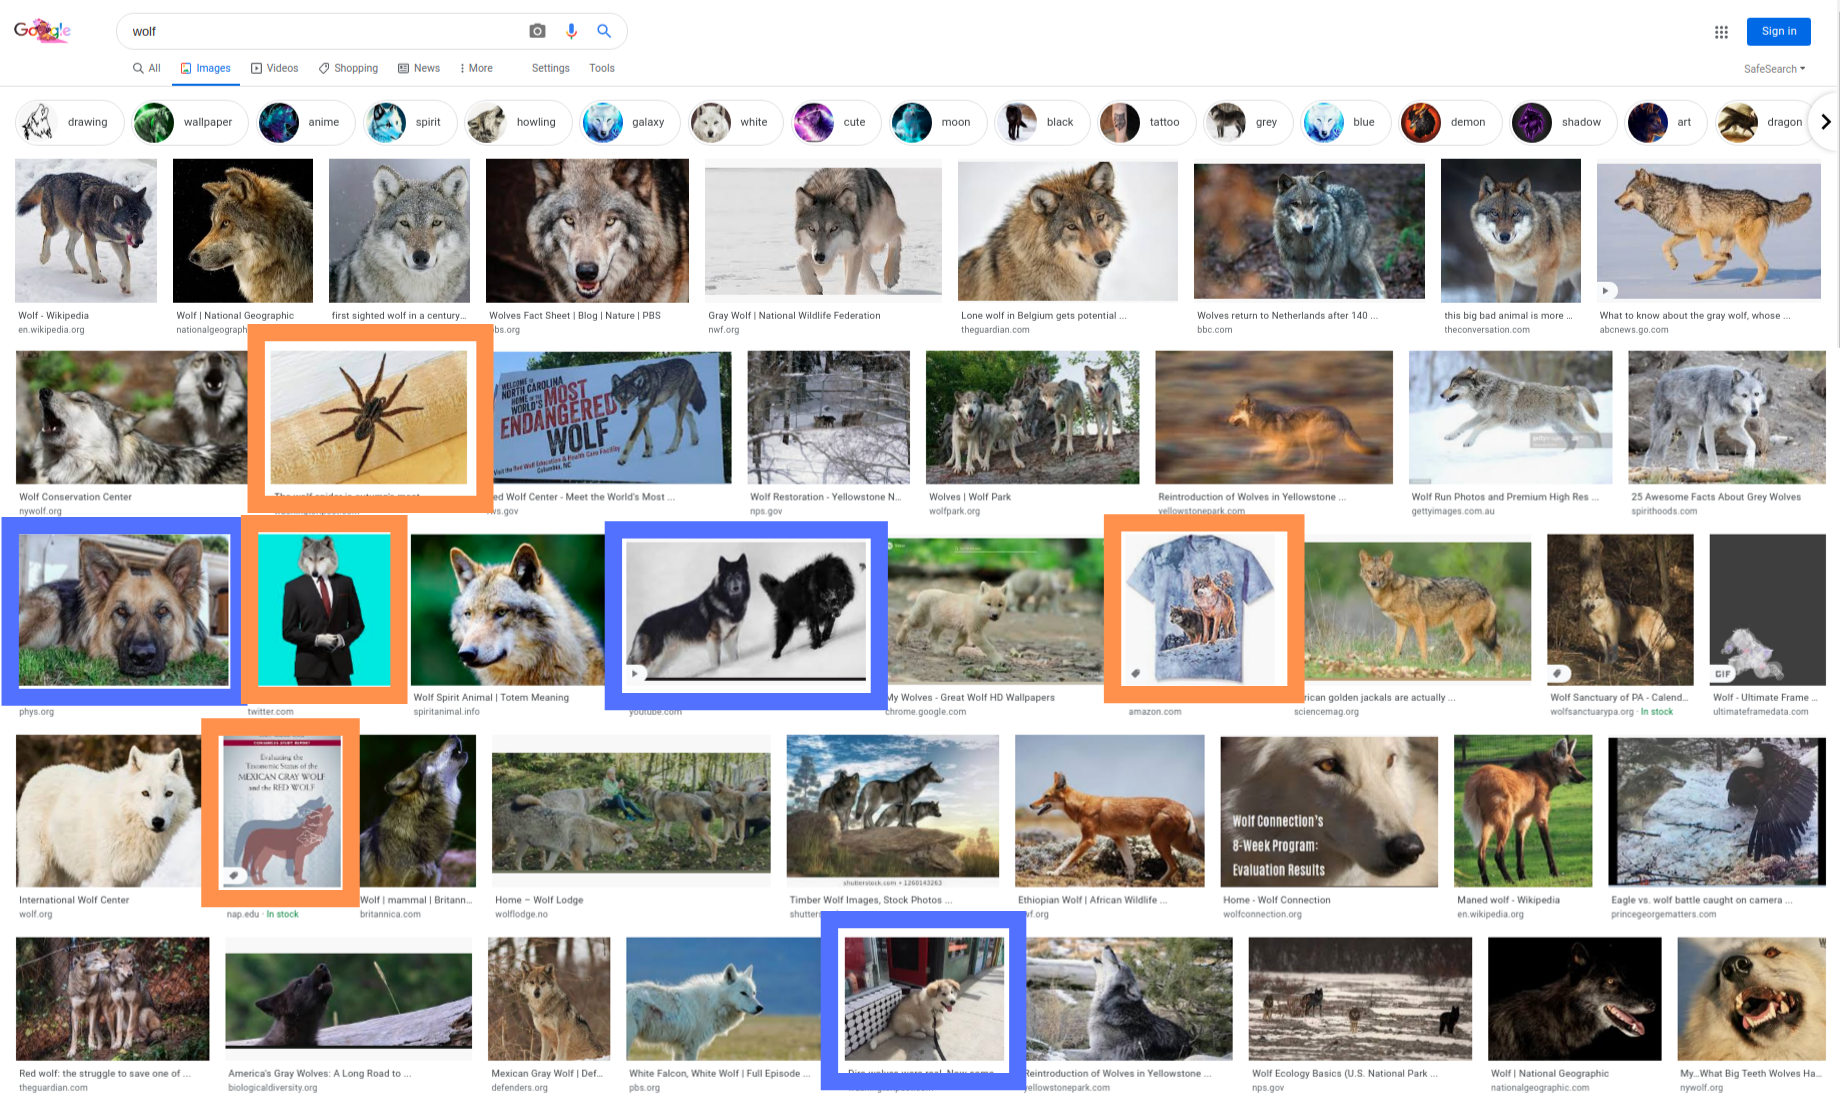
\includegraphics[width=0.8\textwidth]{images/wolfsearch.png}
    \caption{wolf-vs-dog二元分类器数据的搜索引擎查询的结果。这里使用的搜索关键字是 “狼”。由一个橙色边框包围的图像是开集噪声 (即既不是狼也不是狗),被蓝色边框包围的是闭集噪声(即标签上是狼,但实际上是狗)。}
    \label{fig1}
\end{figure}

在本文中,我们提出了一种新的基准评价来解决有噪声的标签学习问题,该问题由一个闭集噪声
和开集噪声的组合组成。这个提出的基准评估由三个变量定义:
1)标签噪声在训练集中所占的总比例,用$\rho \in [0,1]$表示;
2)标签噪声样本集中闭集标签噪声的比率,使用$\omega \in [0,1]$表示;
(这表示了整个训练集中有$\rho \times \omega $比例的样本含有闭集标签噪声,并且有
$\rho \times (1 - \omega) $比例的样本含有开集标签噪声)
3)开集噪声数据的来源。
注意这种设定同时是两种标签噪声的泛化。因为如果 $\omega \in \{0,1\}$,则样本可以被
破坏而具有其中的一种噪声。

最先进的(SOTA)方法旨在解决闭集噪声标签问题,其重点是识别不正确注释的样本,
并使用半监督学习(SSL)方法,更新它们的标签的[14]用于下一次训练迭代。这种策略
很可能在开集问题中失败,因为它假设每个训练样本的真实标签都在研究类别中存在,
但事实并非如此。 另一方面,解决开集噪声问题的主要方法[24]重点在学习过程中,
识别噪声样本并降低其权值。这种策略在闭集问题上效率很低 ,因为闭集的噪声样本在SSL阶段
仍然很有意义。因此,为了在存在闭集和开集噪声样本的情况下具有鲁棒性,
学习算法必须能够识别影响每个训练样本的标签噪声类型。根据类型,如果是闭集标签噪声样本,
则更新标签,如果是开集标签噪声样本则减少其权重。为了实现这一目标,我们提出了一种新的学习算法 ,
名为EvidentialMix (EDM),见图\ref{fig2}。我们提出的算法的关键贡献如下:
\begin{itemize}
    \item EDM能够准确区分干净的、开集和闭集样本,从而允许它根据类型应用不同的
    学习机制。相比之下,以前的方法[14,24]只能将干净样本与噪声样本分离,
    而不能将封闭噪声与开放噪声样本分离。
    \item 我们发现我们的方法可以学习到比以前的研究方法更好的特征表示,如图\ref{fig4}
    中的t-SNE图所示,其中我们的方法对每个已知的标签/类都有一个唯一的聚类,
    而对开集样本给出另一个单独的聚类。相比之下,之前的方法显示出在开集样本上
    很大程度的过拟合,并错误地将它们聚到一个已知的类中。
    \item  我们的实验表明,EDM得到的分类精度,在不同的标签噪声率设定下(包括
    $\omega \in \{0,1\}$这样的极端情况)能够与之前的方法相媲美或能超过他们。
\end{itemize}
\begin{figure}[!htb]
    \centering
    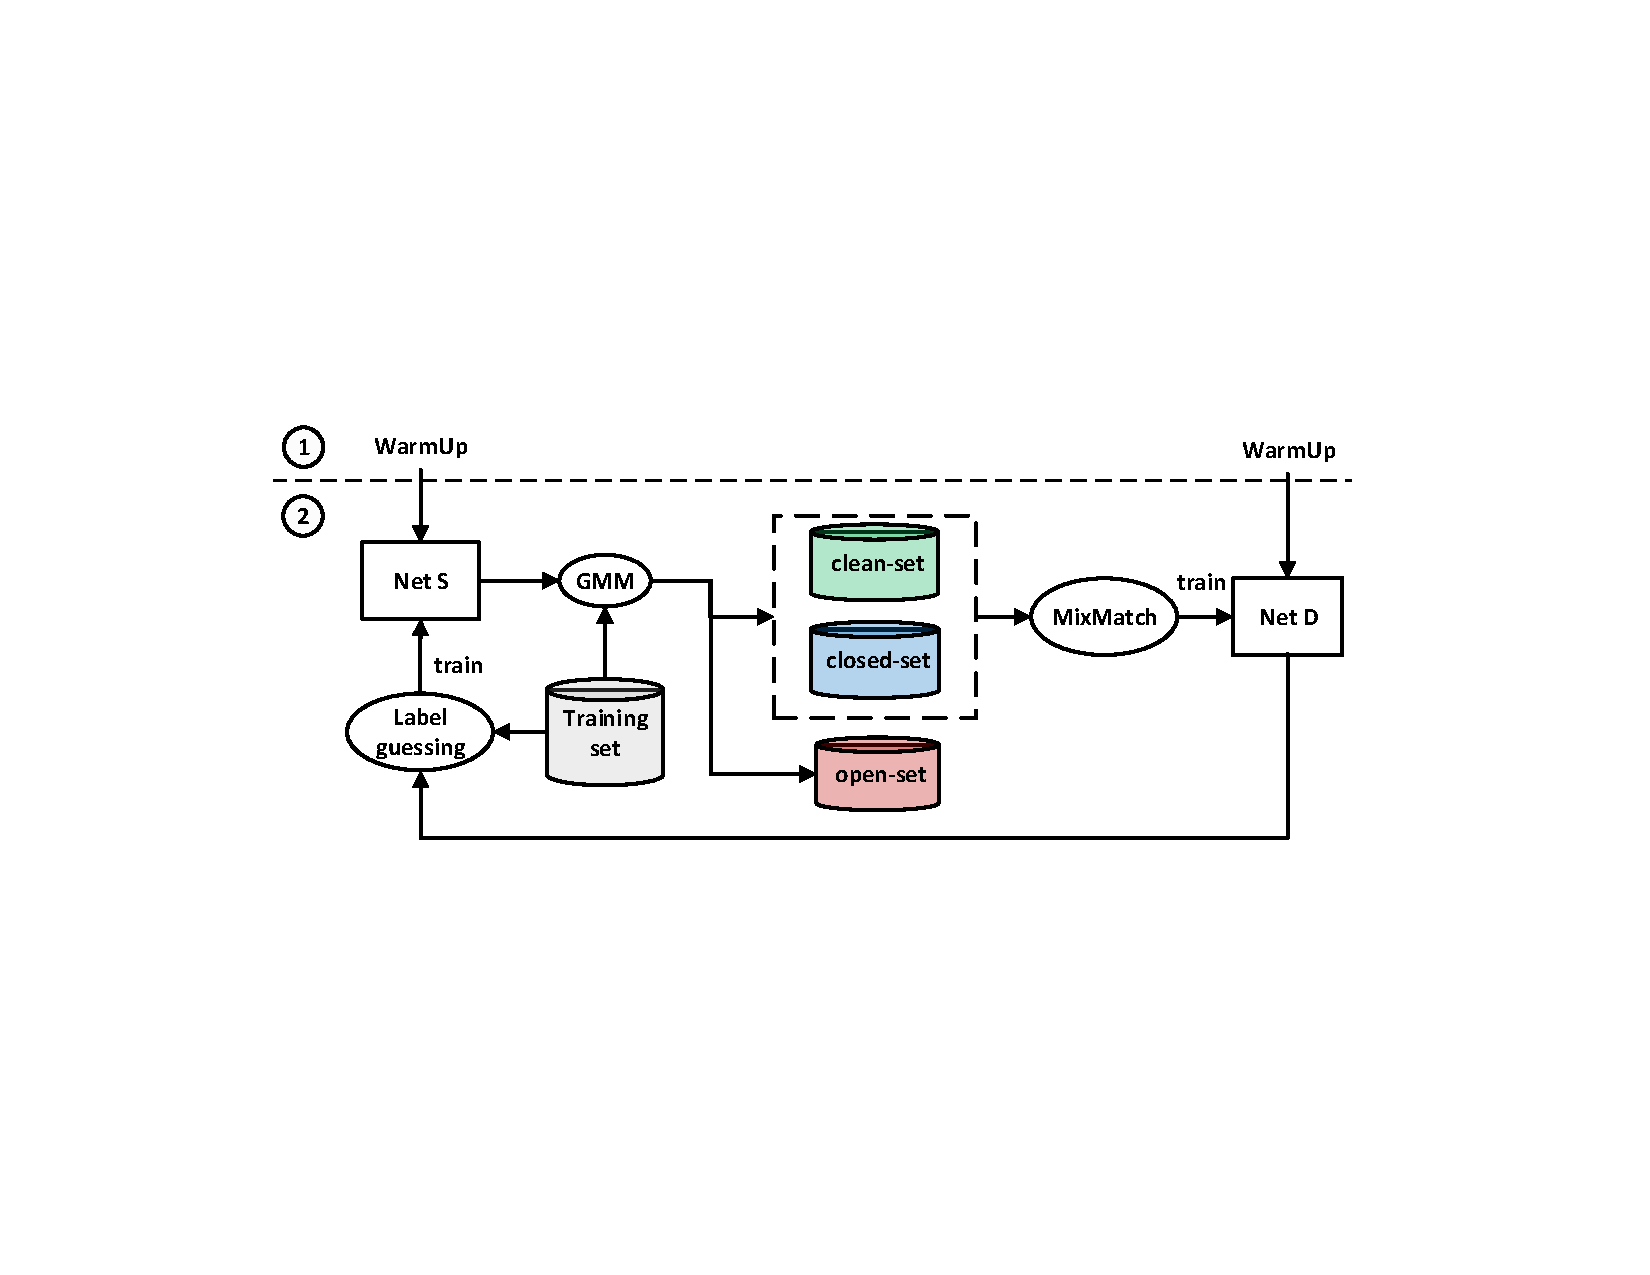
\includegraphics[width=0.8\textwidth]{images/diagrams/EDM_diagram_color6.pdf}
    \caption{我们提出的方法EvidentialMix依赖于两个
    网络,NetD和NetS。这两种模型最初都是使用一个简单的训练机制
    进行几个epoch(见(1)WarmUp)的训练,该机制不包含任何处理标签噪声的方法。接下来在
    (2)中,我们在NetS的样本损失上拟合一个$\psi$-分量高斯混合模型(GMM),以便将
    训练集分离为干净的、闭集和开集样本。在
    这之后,使用SSL学习机制[14]训练NetD,但只使用
    预测的干净和闭集样本。最后,NetS在整个训练集上进行
    训练,以使用NetD估计的标签最小化主观逻辑损失[21],并且
    (2)中的过程重复。}
    \label{fig2}
\end{figure}

\section{先前的研究}
人们对标签噪声设定下深度学习分类建模问题的研究越来越感兴趣。对于
闭集噪声,Reed 等人[19]提出了最早的方法之一,使用转移矩阵来学习标签如何在不同类别
之间切换。转移矩阵在不同的方法中被进一步探索[18,5],但它们都没有显示出有竞争力的结果,
可能是因为它们不包括识别和处理含有噪音标签的样品的机制。数据增广方法[27]相继被
闭集标签噪声方法探索过,其思想是数据增广可以自然增加对噪声标号的训练鲁棒性。
元学习是另一种在闭集噪声标签问题中探索的技术[15,20],但由于需要干净的验证数据集或
人工的新训练任务,这项技术相对来说尚未被探索。研究者也探索了利用课程学习
(CL)[7]解决封闭集问题的方法,在训练过程中根据训练样本的损失值,动态地对训练样本
进行重新标记。该方法已经扩展成多模型训练方法[17,25],目的是聚焦到损失小的样本的训练上,
这些样本被多个模型不一致地分类。最近,Kim等人[9]研究了使用消极学习显式识别噪声样本,
获得了有竞争力的结果。另一种处理标签噪声的重要方法是Tarvainen等人[23]提出的模型集成。
利用具有鲁棒性的生成分类器(RoG)来提高判别分类器的性能的方法在Lee et al.[13]已经
进行了研究,他们从训练好的判别模型的几个层中提取特征,构建鲁棒的线性判别集成模型。
实际上,这种方法有可能提高任何方法的性能,并且已经接连在闭集和开集噪声场景中进行了测试。

开集标签噪声学习直到最近才被wang 等人[24]研究,其思想是识别出含有噪声标签的
样本,并在训练过程中减少它们的权重,因为它们几乎可以肯定属于一个不在训练标签集合中的
类别。鉴于他们的方法是唯一明确处理开集噪声的方法,他们的方法是解决开集标签噪声学习的
主要基准。

目前用于闭集标签噪声学习的SOTA方法是SELF[22]和DivideMix[14]——它们都结合了上述的
多种方法。SELF[22]结合了模型集成、重标记、噪声样本识别和数据增强;
而DivideMix[14]使用了多模型训练、噪声样本识别和数据增强[1]。这两种方法很容易
受到开集噪声的影响,因为它们假设训练样本必须属于某个训练类别——这个假设对于开集噪声来说
是不正确的。
\section{方法}
\subsection{问题定义}
我们定义训练集为$\mathcal{D}=\{(\mathbf{x}_i,\mathbf{y}_i)\}_{i=1}^{|\mathcal{D}|}$,
其中RGB图像为$\mathbf{x}:\Omega \rightarrow \mathbb{R}^3$ ($\Omega$ 表示图像晶格)。
训练标签集合用$\mathcal{Y}$表示,形成了$|\mathcal{Y}|$维度下的标准基。
$\mathbf{y} \in \{0,1\}^{|\mathcal{Y}|}$ ($\sum_{c=1}^{|\mathcal{Y}|}\mathbf{y}(c)=1$,
表示是一个多分类问题)。注意$\mathbf{y}_i$表示的是$\mathbf{x}_i$的噪声标签,潜在的
真实标签用$\mathbf{y}^{*}_i$表示。

对于\textbf{闭合标签噪声问题,噪声率}为$\zeta \in [0,1]$,我们假定
$(\mathbf{x}_i,\mathbf{y}_i) \in \mathcal{D}$以概率$1-\zeta$被标记为
$\mathbf{y}_i = \mathbf{y}^*_i$ ,并以$\zeta$概率被标记为$\mathbf{y}_i \sim r(\mathcal{Y})$,
$r(\mathcal{Y},\theta_r)$表示一个随机函数,从$\mathcal{Y}$选择一个标记,由一个特定
分布以及其参数$\theta_r$控制。

对于\textbf{开集标签噪声问题,噪声率}为$\eta \in [0,1]$,我们需要定义一个新的训练集
$\mathcal{D'}$(满足$\mathcal{D'} \cap \mathcal{D} = \emptyset$)。其中
$\mathcal{D'}$的标签集合用$\mathcal{Y'}$表示(满足$\mathcal{Y'} \cap \mathcal{Y} = \emptyset$)
——这意味着在$\mathcal{D'}$中的图像不再具有$\mathcal{Y}$中的标签。再这样的开集学习问题中,
有$1-\eta$比例的样本从$(\mathbf{x}_i,\mathbf{y}_i) \in \mathcal{D}$且$\mathbf{y}_i=\mathbf{y}^{*}_i$的
样本中抽取。另外$\eta$比例的样本从$(\mathbf{x}_i,\mathbf{y}_i) \in \mathcal{D}$且
$\mathbf{y}_i  \sim r(\mathcal{Y},\theta_r)$的样本中抽取。

对于\textbf{混合的开集和闭集标签噪声问题,噪声率}为$\rho,\omega \in [0,1]$,
混合了上述两种噪声定义。更具体地,$1 - \rho$比例的训练集包含图像$(\mathbf{x}_i,\mathbf{y}_i) \in \mathcal{D}$,标记为
$\mathbf{y}_i = \mathbf{y}_i^{*}$,然而$\omega \times \rho$比例的样本采样自
$(\mathbf{x}_i,\mathbf{y}_i) \in \mathcal{D}$,且标签为$\mathbf{y}_i  \sim r(\mathcal{Y},\theta_r)$。
$(1 - \omega) \times \rho$比例的样本来自集合$\mathcal{D}'$,
且被标记为$\mathbf{y}_i  \sim r(\mathcal{Y},\theta_r)$。

\subsection{噪声分类}
处理这个问题时的主要障碍是需要识别闭集和开集噪声样本,因为它们必须用不同的方法处理。
一种可能的方法是将闭集样本与置信度高而分类错误时[14]计算出的高损失相关联,
将开集样本与不确定的分类相关联。为了实现这一点,我们提出使用主观逻辑(SL)损失函数[21],
依赖于证据推理理论和SL来量化分类不确定性。SL损失利用Dirichlet分布来代表主观意见,
编码信念和不确定性。使用SL损失进行训练的网络试图将预测后验的参数作为Dirichlet密度函数的输出
进而对训练样本进行分类。对于给定样本的输出结果被认为是在一组类别标签上对该样本进行
分类的证据。图\ref{fig3}显示了使用SL损失训练的网络中样本的损失分布。很容易观察到干净、闭集
和开集噪声样本之间的区别。
\begin{figure}[h]
    \centering
    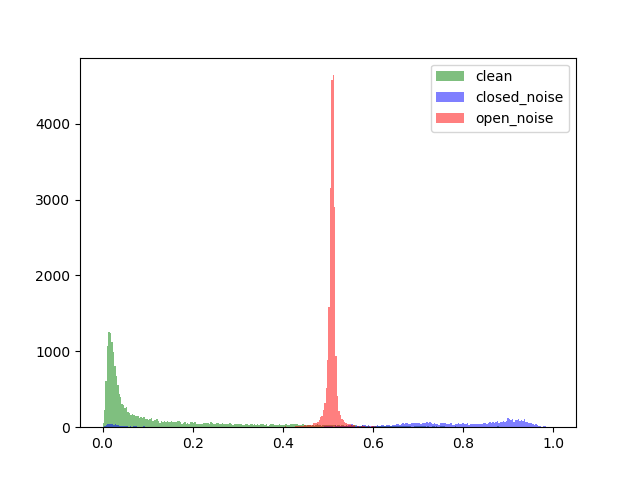
\includegraphics[width=0.5\textwidth]{images/textbook.png}
    \caption{预热阶段过后,使用SL损失函数时每个样本的损失分布。其中全部噪声比率$\rho = 0.6$,闭合噪声比率$\omega = 0.25$(也就是开集噪声比率为$1-\omega = 0.75$)。$\mathcal{D}$为CIFAR-10,$\mathcal{D}'$为ImageNet32。}
    \label{fig3}
\end{figure}
\subsection{EvidentialMix}
我们提出的EvidentialMix方法同时训练两个网络:使用SL loss[21]的NetS、
使用SSL训练机制和DivideMix(DM) loss[14]的NetD。广义地说,SL损失估计分类不确定性
的能力允许NetS将训练集划分为干净集、开集和闭集噪声样本。预测的干净样本和闭集样本
随后被用来配合MixMatch(如[14]所述)训练NetD,而预测的开集噪声样本在当前epoch被丢弃。
在此之后,NetD重新标记整个训练数据集(包括预测的开集样本),然后用来训练NetS。

随着NetS不断地从NetD预测的标签中学习,它可以更好地将数据分成三个集合。
这是因为NetD预测的标签在训练过程中变得更加准确,因为它只在干净样本和闭集样本上进行
训练,而从不训练被预测为开集的样本。这两个网络相互补充,从而对组合的闭集和开集噪声问题
产生准确的分类结果。下面列出了详细的解释,而算法1详细地描述了整个训练过程。

\begin{algorithm}[H]
    \caption{EvidentialMix(EDM)}%算法名字
    \LinesNumbered %要求显示行号
    \KwIn{$\mathcal{D}=\{(\mathbf{x}_i,\mathbf{y}_i)\}_{i=1}^{|\mathcal{D}|}$, number of augmentations $M$, temperature sharpening $T$, loss weights $\lambda^{(\mathcal{U})}$ and $\lambda^{(reg)}$, MixMatch parameter $\alpha$, number of epochs $E$.}%输入参数
    \KwOut{output result}%输出
    $f_{\theta^{(D)}}(c|\mathbf{x}), f_{\theta^{(S)}}(c|\mathbf{x})$ = WarmUp($\mathcal{D}$)\;
    \While{$e < E$}{
  $\mathcal{W},\mathcal{W}^{\text{op}},\mathcal{W}^{\text{cl}}$ = GMM($\mathcal{D}, f_{\theta^{(S)}}(c|\mathbf{x})$) \\
  \tcp{Train NetD}
  $\mathcal{X} = \{ (\mathbf{x}_i, \mathbf{y}_i, w_i) | (\mathbf{x}_i, \mathbf{y}_i, w_i) \in (\mathcal{D},\mathcal{W}) , w_i >   \max(w_i^{\text{op}},w_i^{\text{cl}})\}$ \\  
  $\mathcal{U} = \{\mathbf{x}_i| (\mathbf{x}_i, \mathbf{y}_i) \in \mathcal{D} , w_i^{\text{cl}} >   
  \max(w_i,w_i^{\text{op}})\}$ \\
  \For{iter=1 \textbf{to} num\_iters}   
        {
            $\{(\mathbf{x}_b, \mathbf{y}_b, w_b)\}_{b=1}^{B} \subset \mathcal{X}$ \tcp{randomly pick $B$ samples from $\mathcal{X}$}
            
            $\{\mathbf{u}_b\}_{b=1}^{B} \subset \mathcal{U}$ \tcp{randomly pick $B$ samples from $\mathcal{U}$}
            
            \For{b=1 \textbf{to} B}   
            {
                \For{m=1 \textbf{to} M}   
                {
                    $\hat{\mathbf{x}}_{b,m}$ = DataAugment($\mathbf{x}_b$)  \\
                    $\hat{\mathbf{u}}_{b,m}$ = DataAugment($\mathbf{u}_b$) \\
                }
                \For{c=1 \textbf{to} $|\mathcal{Y}|$}
                {
                    $\mathbf{p}_b(c) = \frac{1}{M}\sum_m p_{\theta^{(D)}}(c|\hat{\mathbf{x}}_{b,m})$\\
                    $\mathbf{q}_b(c) = \frac{1}{M}\sum_m p_{\theta^{(D)}}(c | \hat{\mathbf{u}}_{b,m})$ \\
                }
                $\hat{\mathbf{y}}_b$ = TempSharpen$_{T}(w_b \mathbf{y}_b + (1-w_b)\mathbf{p}_b)$ \\
                $\hat{\mathbf{q}}_b$ = TempSharpen$_{T}(\mathbf{q}_b)$ \\
            }
            $\hat{\mathcal{X}} = \{(\hat{\mathbf{x}}_{b,m},\hat{\mathbf{y}}_b)\}_{b \in (1,...,B), m \in (1,...,M)}$ \\
            $\hat{\mathcal{U}} = \{(\hat{\mathbf{u}}_{b,m},\hat{\mathbf{q}}_b) \}_{b \in (1,...,B), m \in (1,...,M)}$ \\
            $\mathcal{X}', \mathcal{U}' = \text{MixMatch}_{\alpha}(\hat{\mathcal{X}},\hat{\mathcal{U}}$) \\
            $\theta^{(D)} = \text{SGD}(\mathcal{L}^{(D)},\theta^{(D)},\mathcal{X}', \mathcal{U}')$ \\
        }
        \tcp{Train NetS}
        \For{i=1 \textbf{to} $|\mathcal{D}|$}
        {
            $\hat{c}_i = \arg\max_{c \in \mathcal{Y}} \left [ (w_i^{\text{cl}}) p_{\theta^{(D)}}(c|\mathbf{x}_i) +
                (1-w_i^{\text{cl}}) \mathbf{y}_i(c)) \right ]$\\
            $\hat{\mathbf{y}}_i = \text{onehot}(\hat{c}_i) $\\
        }
        $\theta^{(S)} = SGD(\mathcal{L}^{(S)},\theta^{(S)},\{ (\mathbf{x}_i,\hat{\mathbf{y}}_i) \}_{i=1}^{|\mathcal{D}|}$) \\
 }
 \label{alg:EDM}
 \caption{EvidentialMix (EDM)}
    % \For{condition}{
    %     only if\;
    %     \If{condition}{
    %     1\;
    %     }
    % }
    % \While{not at end of this document}{
    %     if and else\;
    %     \eIf{condition}{
    %         1\;
    %     }{
    %         2\;
    %     }
    % }
    % \ForEach{condition}{
    %     \If{condition}{
    %         1\;
    %     }
    % }
\end{algorithm}

\subsection{实现}



\section{实验}

% 噪声分布对比图
\begin{figure*}[t]
    \centering
    \hspace*{0mm}{\scriptsize \hspace{5mm} ImageNet32 \hspace{45mm} CIFAR-100}  \\
    \noindent \hspace*{5mm}  \rule{5cm}{0.5pt} \hspace{7mm} \rule{5cm}{0.5pt}
    \\
    % \hspace*{9mm}{\scriptsize \hspace{1mm}\asmall \hspace{13mm} \amedium \hspace{15mm} \alarge \hspace{14mm} \fsmall \hspace{2.5mm}}\\
    \begin{subfigure}{.18\textwidth}
      \centering
      % include first image
      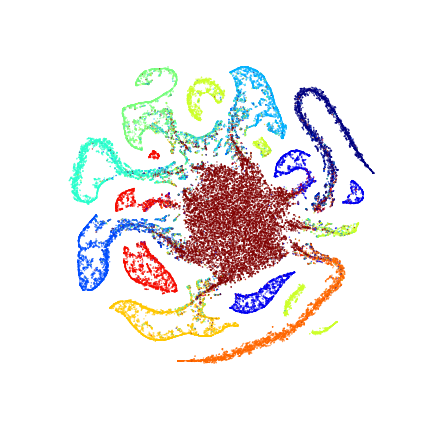
\includegraphics[width=\linewidth]{images/tsne/tsne_ROG_imagenet32.png}
      \caption*{RoG~}
    \end{subfigure}
    \begin{subfigure}{.18\textwidth}
      \centering
      % include second image
      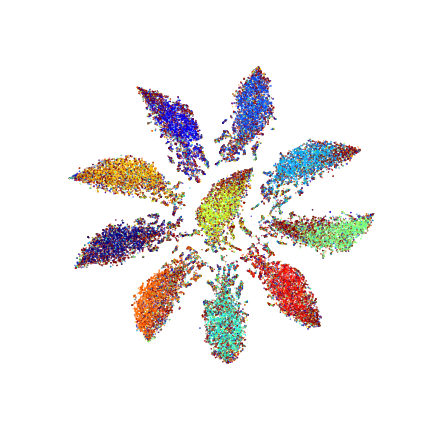
\includegraphics[width=\linewidth]{images/tsne/tsne_ILON_imagenet32.png}
      \caption*{ILON~}
    \end{subfigure}
    \begin{subfigure}{.18\textwidth}
      \centering
      % include second image
     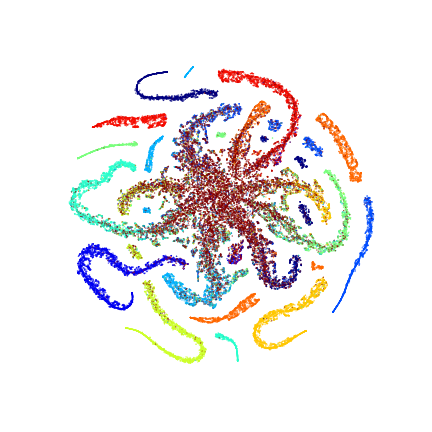
\includegraphics[width=\linewidth]{images/tsne/tsne_ROG_cifar100.png}
     \caption*{RoG~}
    \end{subfigure}
    \begin{subfigure}{.18\textwidth}
      \centering
      % include second image
      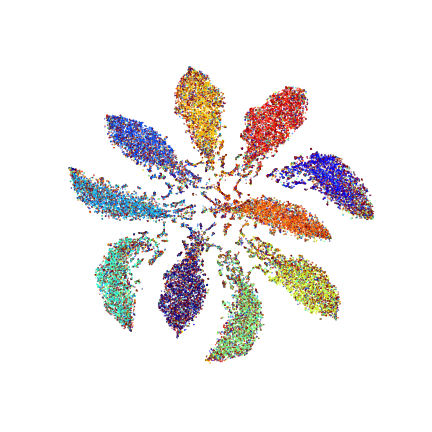
\includegraphics[width=\linewidth]{images/tsne/tsne_ILON_cifar100.png}
      \caption*{ILON~}
    \end{subfigure}
    \\
    \begin{subfigure}{.18\textwidth}
      \centering
      % include first image
      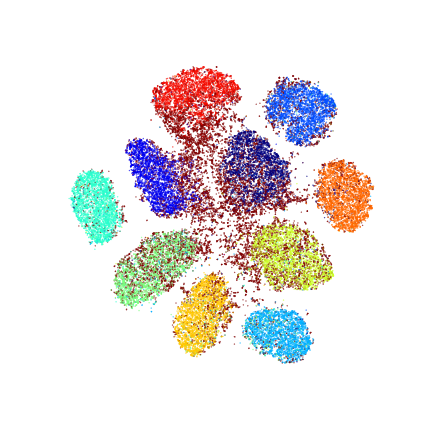
\includegraphics[width=\linewidth]{images/tsne/tsne_DM_imagenet32.png} 
      \caption*{DivideMix~}
    \end{subfigure}
    \begin{subfigure}{.18\textwidth}
      \centering
      % include second image
      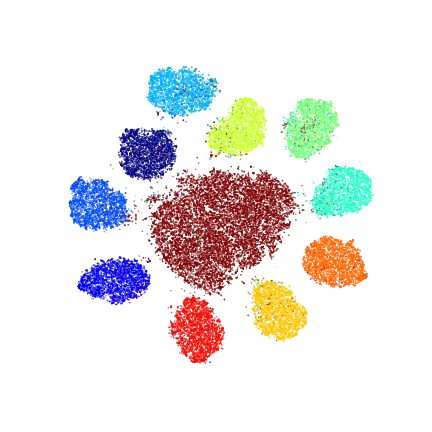
\includegraphics[width=\linewidth]{images/tsne/tsne_EDM_imagenet32_D.png}
      \caption*{EDM [ours]}
    \end{subfigure}
    \begin{subfigure}{.18\textwidth}
      \centering
      % include second image
      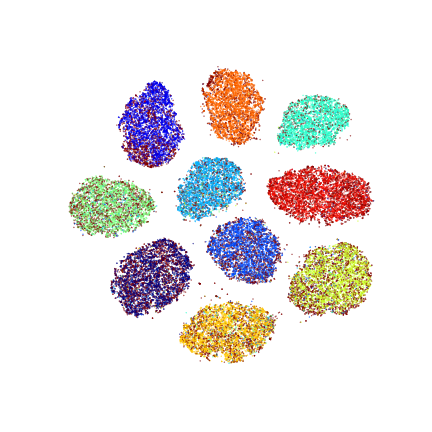
\includegraphics[width=\linewidth]{images/tsne/tsne_DM_cifar100.png}
      \caption*{DivideMix~}
    \end{subfigure}
    \begin{subfigure}{.18\textwidth}
      \centering
      % include second image
      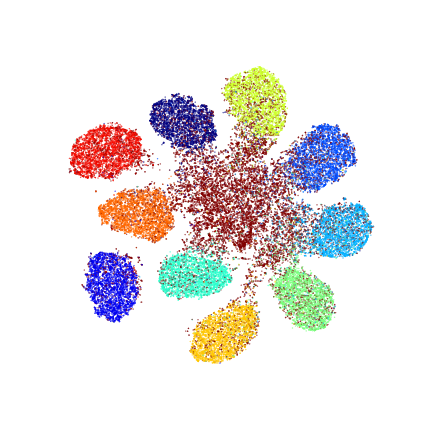
\includegraphics[width=\linewidth]{images/tsne/tsne_EDM_cifar100_D.png}
      \caption*{EDM [ours]}
    \end{subfigure}
    \caption{相关方法和我们提出的EDM方法的TSNE图,其中整体的噪声率是$\rho = 0.6$,
    开集噪声的比率是$\omega = 0.5$,CIFAR-100和ImageNet32表示开集数据集。其中\textbf{棕色}
    样本表示开集噪声样本,其他颜色表示真实的CIFAR-10类别。
    }
    \label{fig4}
\end{figure*}
% 损失分布图
\begin{figure*}[t]
    \centering
    \hspace*{8mm}{\scriptsize EDM [ours] \hspace{50mm} DivideMix }  \\
    \noindent  \rule{5cm}{0.5pt} \hspace{12mm} \rule{5cm}{0.5pt}
    \\
    
    \begin{subfigure}{.18\textwidth}
      \centering
      % include first image
      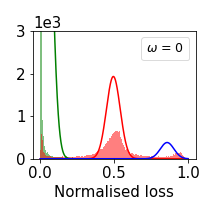
\includegraphics[width=\linewidth]{images/loss_dist/EDM_0.6_1.00_cifar100.png} 
    \end{subfigure}
    \begin{subfigure}{.18\textwidth}
      \centering
      % include second image
      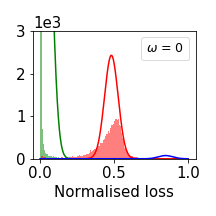
\includegraphics[width=\linewidth]{images/loss_dist/EDM_0.6_1.00_imagenet32.png} 
    \end{subfigure}
    \begin{subfigure}{.18\textwidth}
      \centering
      % include second image
      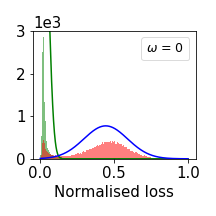
\includegraphics[width=\linewidth]{images/loss_dist/DM_0.6_1.00_cifar100.png} 
    \end{subfigure}
    \begin{subfigure}{.18\textwidth}
      \centering
      % include second image
      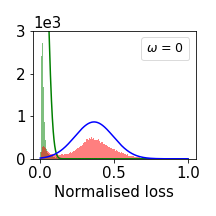
\includegraphics[width=\linewidth]{images/loss_dist/DM_0.6_1.00_imagenet32.png} 
    \end{subfigure}
    \\
    \begin{subfigure}{.18\textwidth}
      \centering
      % include first image
      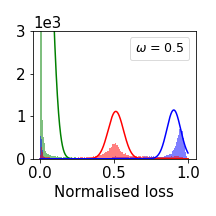
\includegraphics[width=\linewidth]{images/loss_dist/EDM_0.6_0.50_cifar100.png} 
    \end{subfigure}
    \begin{subfigure}{.18\textwidth}
      \centering
      % include second image
      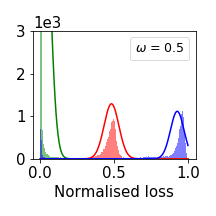
\includegraphics[width=\linewidth]{images/loss_dist/EDM_0.6_0.50_imagenet32.png} 
    \end{subfigure}
    \begin{subfigure}{.18\textwidth}
      \centering
      % include second image
      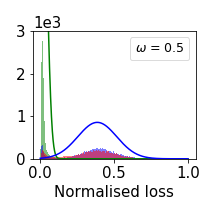
\includegraphics[width=\linewidth]{images/loss_dist/DM_0.6_0.50_cifar100.png} 
    \end{subfigure}
    \begin{subfigure}{.18\textwidth}
      \centering
      % include second image
      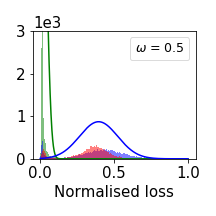
\includegraphics[width=\linewidth]{images/loss_dist/DM_0.6_0.50_imagenet32.png} 
    \end{subfigure}
    \\
    \begin{subfigure}{.18\textwidth}
      \centering
      % include first image
      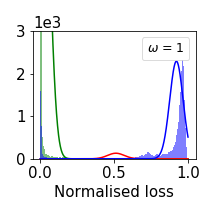
\includegraphics[width=\linewidth]{images/loss_dist/EDM_0.6_0.00_cifar100.png} 
    \end{subfigure}
    \begin{subfigure}{.18\textwidth}
      \centering
      % include second image
      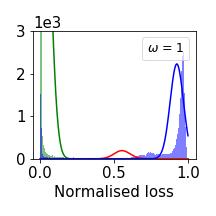
\includegraphics[width=\linewidth]{images/loss_dist/EDM_0.6_0.00_imagenet32.png} 
    \end{subfigure}
    \begin{subfigure}{.18\textwidth}
      \centering
      % include second image
      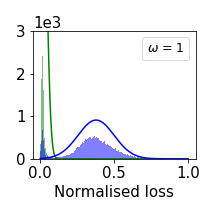
\includegraphics[width=\linewidth]{images/loss_dist/DM_0.6_0.00_cifar100.png} 
    \end{subfigure}
    \begin{subfigure}{.18\textwidth}
      \centering
      % include second image
      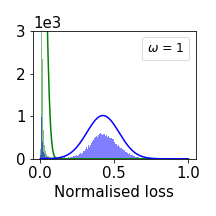
\includegraphics[width=\linewidth]{images/loss_dist/DM_0.6_0.00_imagenet32.png} 
    \end{subfigure}
    \\
    \begin{subfigure}{\textwidth}
      \centering
      % include second image
      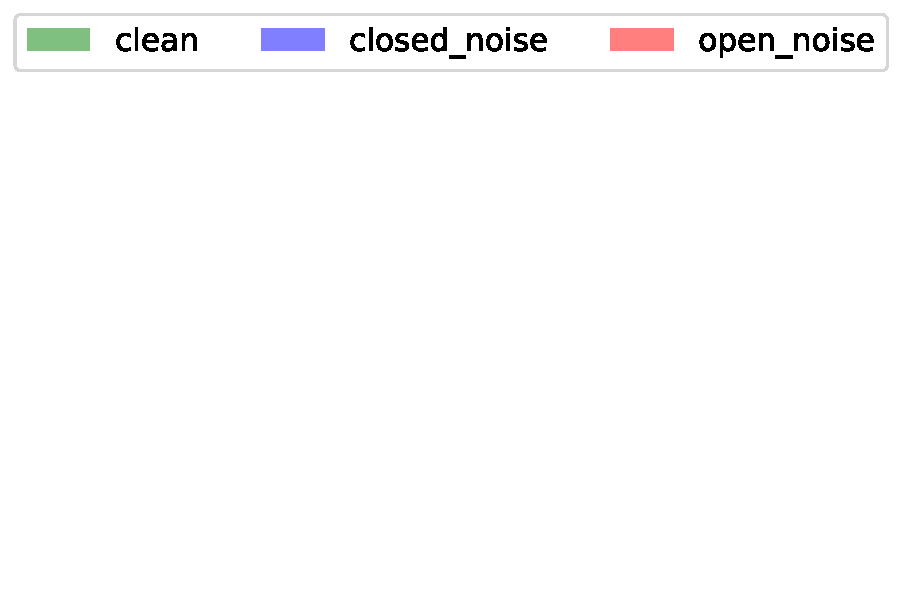
\includegraphics[width=0.4\linewidth]{images/loss_dist/legend.pdf} 
    \end{subfigure}
    \caption{Per-sample loss distributions for the open-set (orange), closed set (blue) and clean set (green) samples produced by EDM (left) and DivideMix (right) at epoch $e=100$, where $\rho=0.6$ and $\omega \in \{0,0.5,1\}$, with open-set datasets $\in$ \{CIFAR-100, ImageNet32\}.  We also show the estimated GMM posterior probabilities for the clean, open-set and closed-set noise samples using our EDM, and for the clean and noisy samples using DivideMix~.}
    \label{fig5}
\end{figure*}
\subsection{混合的开集和闭集标签噪声基准}
\subsection{相关的对比方法}
\subsection{结果和讨论}
\section{结论}

\bibliographystyle{plain}
\bibliography{ref}
\end{document}



